\section{Geometry and magnetic-transport calculation}\label{app:v505-geometry}
\subsection{Two-body decay and laboratory acceptance}
\label{v571:kinematics}

The beam energy controls the angular separation of the electron and positron
from a boosted dark photon.  We first consider a prompt $A'\to e^+e^-$ decay
at the target, with the parent directed along the beam axis $z$.  In units with
$c=1$, let $m$ denote the parent mass and write its laboratory energy as
$E_A=xE_{\rm beam}$, where $x$ is the fraction of the beam energy carried by
the parent.  At fixed $m$ and $x$, the boost and daughter rest-frame momentum are
\begin{equation}
  \gamma=\frac{E_A}{m},\qquad
  \beta=\sqrt{1-\frac{m^2}{E_A^2}},\qquad
  E_* = \frac{m}{2},\qquad
  p_* = \sqrt{\frac{m^2}{4}-m_e^2},
  \label{v571:boost}
\end{equation}
with $2m_e\leq m<E_A$.  Define $c_*=\cos\theta_*$ and let $\phi_*$ be the
rest-frame azimuth measured from the horizontal $x$ axis.  The two rest-frame
four-vectors and their laboratory components are
\begin{equation}
  p_{\pm}^{*\mu}
    =\left(\frac m2,\ \pm p_*\sqrt{1-c_*^2}\cos\phi_*,\
       \pm p_*\sqrt{1-c_*^2}\sin\phi_*,\ \pm p_*c_*\right),
       \label{v571:rest-vectors}
\end{equation}
\begin{align}
  E_\pm&=\gamma\left(\frac m2\pm\beta p_*c_*\right),&
  p_{z,\pm}&=\gamma\left(\frac{\beta m}{2}\pm p_*c_*\right),
       \label{v571:lab-vectors}\\
  p_{x,\pm}&=\pm p_*\sqrt{1-c_*^2}\cos\phi_*,&
  p_{y,\pm}&=\pm p_*\sqrt{1-c_*^2}\sin\phi_* .
       \label{v571:transverse-vectors}
\end{align}
The signs label the opposite daughter directions.  For a forward daughter,
its polar angle and vertical projected angle are respectively
\begin{equation}
  \tan\theta_\pm=\frac{p_*\sqrt{1-c_*^2}}{p_{z,\pm}},\qquad
  \tan\theta_{y,\pm}=\frac{p_{y,\pm}}{p_{z,\pm}}.
  \label{v571:angles}
\end{equation}
The energy fractions are $E_\pm/E_A=(1\pm\beta\rho c_*)/2$, where
$\rho=\sqrt{1-4m_e^2/m^2}$.  They approach the momentum fractions only when
the daughters are ultrarelativistic.  Thus fixing $x$ fixes the pair energy,
while the decay angle still determines how that energy is shared.

\subsubsection{Equal-sharing mass scales}
\label{v571:equal-sharing}
For $c_*=0$, both daughters have energy $E_A/2$ and the same polar angle
$\theta$; their opening angle is $2\theta$.  The exact invariant-mass relation is
\begin{equation}
  m^2=E_A^2\sin^2\theta+4m_e^2\cos^2\theta
  \quad\longrightarrow\quad
  m\simeq xE_{\rm beam}\sin\theta
  \simeq xE_{\rm beam}\theta .
  \label{v571:equal-sharing-mass}
\end{equation}
The first approximation neglects the electron mass and the second assumes a
small angle.  In the vertical decay plane, $|\sin\phi_*|=1$, this gives the
mass scale associated with a specified vertical angle.  For a general decay,
the small-angle, relativistic relation is instead
$m^2\simeq E_+E_-\theta_{+-}^2$, with
$\theta_{+-}$ the daughter opening angle.  Unequal sharing therefore changes
the correspondence between a mass and either single-track angle.

A vertical beam gap excludes tracks close to the beam \emph{plane}; a polar
cone excludes tracks close to the beam \emph{axis}.  Their acceptances differ
because $|\tan\theta_y|=\tan\theta\,|\sin\phi_*|$.  In particular, an outer
vertical edge gives an upper equal-sharing mass scale only in the specified
vertical plane.  With unrestricted azimuth it does not, by itself, give an
upper mass cutoff.  Horizontal sensor boundaries and magnetic bending must
also be considered before interpreting an endpoint as detector acceptance.

\subsubsection{Normalized decay fraction through the tracker}
\label{v571:acceptance}
For the conditional angular calculation, we use a transverse-vector decay
distribution in the relativistic-daughter approximation, with uniform
azimuth:
\begin{equation}
  w(c_*)=\frac38(1+c_*^2),\qquad
  \mathcal A(m,x)=\int_{-1}^{1}\!dc_*\,w(c_*)
    \int_0^{2\pi}\!\frac{d\phi_*}{2\pi}\,
    \mathcal I_{\rm geom}(p_+,p_-).
  \label{v571:acceptance-integral}
\end{equation}
Here $\mathcal I_{\rm geom}$ is one when both forward daughters satisfy the
chosen geometrical requirements and zero otherwise.  The integral is
normalized to all decays with that specified polarization, parent energy and
direction.  Finite $m_e$ is retained in the kinematics above; the adopted
angular weight is not an exact threshold or production-polarization model.

For an active sensor rectangle centered at $\boldsymbol r_j$, let
$\boldsymbol n_j$ be its normal, $\boldsymbol a_j,\boldsymbol b_j$ its
orthogonal in-plane unit vectors, and $h_{a,j},h_{b,j}$ its active half-widths.
For the zero-field reference, a straight daughter ray
$\boldsymbol r(t)=\boldsymbol r_0+t\boldsymbol u$,
with $\boldsymbol u=\boldsymbol p/|\boldsymbol p|$, crosses the sensor plane at
\begin{align}
  t_j&=\frac{(\boldsymbol r_j-\boldsymbol r_0)\cdot\boldsymbol n_j}
                {\boldsymbol u\cdot\boldsymbol n_j},&
  \Delta\boldsymbol r_j&=\boldsymbol r_0+t_j\boldsymbol u-\boldsymbol r_j,
  \nonumber\\
  |\Delta\boldsymbol r_j\cdot\boldsymbol a_j|&\leq h_{a,j},&
  |\Delta\boldsymbol r_j\cdot\boldsymbol b_j|&\leq h_{b,j}.
  \label{v571:sensor-intersection}
\end{align}
A geometrical sensor hit requires $t_j>0$, a nonparallel ray, and both bounds.
For station $k$ in a specified detector half, define binary flags
$h_{k,a}$ and $h_{k,s}$ for its axial and stereo views.  Each flag is one if
the ray crosses any active rectangle belonging to that view.  Where hole and
slot sensors are alternatives in one view, their rectangles form a union:
crossing either is sufficient, and that view is counted at most once.
The geometrical counts for one daughter are then
\begin{equation}
  N_{\rm 2D}=\sum_k(h_{k,a}+h_{k,s}),\qquad
  N_{\rm 3D}=\sum_k h_{k,a}h_{k,s}.
  \label{v571:hit-counts}
\end{equation}
Thus a 2D plane hit requires one view, whereas a paired 3D space point
requires both views at the same station and in the same detector half.
These counts are not interchangeable when only one view is crossed:
$N_{\rm 2D}=2N_{\rm 3D}$ holds only if every crossed view has its partner.
The run- and charge-dependent thresholds, including any required inner-plane
hits, are specified in the selection table below.  They enter
$\mathcal I_{\rm geom}$ separately for the electron and positron.
Equation~\eqref{v571:sensor-intersection} gives the analytic crossing for the
zero-field reference. With a magnetic field, the curved daughter trajectory
determines the sensor crossings before the same view and station flags are
evaluated. These counts omit scattering and hit inefficiency.

\begin{samepage}
\paragraph{Magnetic propagation}
\label{v571:magnetic-propagation}
Let $s$ denote path length, $q=+1$ for the positron and $q=-1$ for the
electron, and $\boldsymbol B(\boldsymbol r)$ the static field in the detector
coordinate frame. For momentum in MeV, position in mm and field in tesla,
the transport equations are
\begin{equation}
 \begin{gathered}
  \frac{d\boldsymbol r}{ds}=\boldsymbol u
      =\frac{\boldsymbol p}{|\boldsymbol p|},\qquad
  \frac{d\boldsymbol p}{ds}
      =\kappa q\,\boldsymbol u\times\boldsymbol B(\boldsymbol r),\\[3pt]
  \kappa=0.299792458\ \frac{\mathrm{MeV}}{\mathrm{T\,mm}}.
 \end{gathered}
  \label{v571:magnetic-equations}
\end{equation}
\end{samepage}
The magnetic force is perpendicular to the momentum, so
$d|\boldsymbol p|^2/ds=0$: each daughter's momentum magnitude and energy
remain constant in this transport model. The field changes the trajectory
and the directions at the sensors. The mass labeling the acceptance curves
is the invariant mass of the two momenta at the production vertex, rather
than a mass recomputed from their different local directions downstream.
Energy loss and material scattering require additional physics.

The numerical trajectory crosses sensor plane $j$ at a forward path length
$s_j>0$ satisfying
\begin{equation}
  \bigl[\boldsymbol r(s_j)-\boldsymbol r_j\bigr]\cdot
  \boldsymbol n_j=0.
  \label{v571:curved-crossing}
\end{equation}
The in-plane half-width bounds of Eq.~\eqref{v571:sensor-intersection}
are then tested at $\boldsymbol r(s_j)$. This prescription follows each
charge through the same field and retains the complete finite sensor
geometry. Setting $\boldsymbol B=0$ recovers the straight-ray calculation.
The field map, integration method and numerical checks are specified with
the detector configuration below.

\paragraph{Projected angular reference}

For an illustrative projection, consider symmetric active
vertical intervals $y_{\min,j}\leq |y|\leq y_{\max,j}$ at longitudinal
positions $z_j$, measured from a target at $z_0$.  A straight trajectory from
the target has $y_j=(z_j-z_0)p_y/p_z$.  Requiring each daughter to cross every
chosen interval reduces to a constant slope band
\begin{equation}
  L\equiv\max_j\frac{y_{\min,j}}{z_j-z_0}
    \leq\left|\frac{p_y}{p_z}\right|\leq
  U\equiv\min_j\frac{y_{\max,j}}{z_j-z_0},
  \label{v571:projected-band}
\end{equation}
provided $0\leq L<U$.  This band is a reference for understanding the angular
scales, rather than a replacement for the finite sensor calculation.

The azimuthal integral can be performed explicitly.  At fixed $c_*$, set
$p_T=p_*\sqrt{1-c_*^2}$ and, for $p_T>0$ and $p_{z,+},p_{z,-}>0$, define
\begin{equation}
  q_{\rm low}=\frac{L\max(p_{z,+},p_{z,-})}{p_T},\qquad
  q_{\rm high}=\frac{U\min(p_{z,+},p_{z,-})}{p_T}.
  \label{v571:azimuth-bounds}
\end{equation}
Both daughters pass if $q_{\rm low}\leq |\sin\phi_*|\leq q_{\rm high}$.
Writing $[q]_0^1=\min(1,\max(0,q))$ and $[a]_+=\max(0,a)$, the accepted
azimuthal fraction and the remaining integral are
\begin{equation}
  F_\phi(c_*)=\frac2\pi
    \left[\arcsin\bigl([q_{\rm high}]_0^1\bigr)-
          \arcsin\bigl([q_{\rm low}]_0^1\bigr)\right]_+,\qquad
  \mathcal A_{\rm band}=\int_{-1}^{1}\!dc_*\,w(c_*)F_\phi(c_*).
  \label{v571:azimuth-fraction}
\end{equation}
We set $F_\phi=0$ when either daughter is backward or the nonzero-gap aperture
cannot be reached.  This fraction describes geometry under the stated
assumptions.  A selected mass spectrum additionally depends on production,
beam exposure, energy and direction distributions, trigger, reconstruction
and analysis requirements; it is not a measurement of $\mathcal A(m,x)$.

\subsubsection{A numerical boost example}
For a 90 MeV parent carrying the 2016 beam energy, $E_A=2.30$ GeV,
Eq.~\eqref{v571:boost} gives $\gamma=25.556$ and $\beta=0.999234$.
At equal sharing, $E_+=E_-=1150$ MeV, $p_*=44.997$ MeV and
$p_{z,+}=p_{z,-}=1149.119$ MeV. Each daughter is therefore at
$\theta=39.138$ mrad to the beam; the opening angle is 78.276 mrad.
Rotating the decay azimuth changes its vertical projection while preserving
the pair mass and polar opening. This is why a mass alone does not determine
whether an event crosses the active silicon.

For comparison, the nominal 15 mrad vertical design angle gives, in the
equal-sharing vertical plane at $x=1$ and neglecting $m_e$,
\begin{equation}
 m_{15}\simeq E_{\rm beam}\sin(0.015)
   =\left(15.84,\ 34.50,\ 56.10\right)\ {\rm MeV}
 \label{v571:fifteen-mrad-reference}
\end{equation}
for 2015, 2016 and 2021, respectively. These are reference mass scales;
the 15 mrad gap alone provides no upper mass cutoff.

\subsection{Detector geometry, fields and hit selection}
\label{v571:geometry}
The beam energies are 1.056, 2.30 and 3.74 GeV for 2015, 2016 and 2021,
respectively~\cite{v571:HPS2022,v571:HPS2015,v571:HPS2016}.
The detector input is the committed LCDD geometry in
\texttt{JeffersonLab/hps-java}, fixed to revision
\texttt{473c732d}~\cite{v571:geometry-source}; the complete identifier is saved
in the source manifest.
LCDD contains the active sensor solids and their complete placement hierarchy.
The corresponding compact XML and Java geometry definitions are retained as
supporting sources; a fresh rebuild of those definitions is not assumed to
reproduce the committed alignment exactly.

The selected configurations are
\nolinkurl{HPS-EngRun2015-Nominal-v6-0-fieldmap},
\nolinkurl{HPS-PhysicsRun2016-Pass2} and
\nolinkurl{HPS_Run2021Pass2FEE}. The first is a representative nominal
engineering-run configuration. The second appears in local HPSTR radiative-MC
filenames. The third is explicitly selected by the local 2021 HPSTR simulation
job list, with run 14166 and target $z=0$. Exact alignment and selection
equivalence to the three observed histograms has not been established.

The extracted geometries contain 36, 36 and 40 active silicon rectangles.
Standard sensors have active dimensions
$38.3399\times98.33\times0.32$ mm. The first two 2021 stations instead use
$14.025\times30\times0.20$ mm sensors. There are six station pairs in the
engineering-run layouts and seven in 2021. In the 2021 file, the first station
corresponds to the added physical L0; its axial and stereo planes are staggered,
as are the top and bottom planes. The earliest sensor centers lie near
$z=38$ mm in 2021 and $z=88$ mm in the older layouts. A nominal station
distance of 50 or 100 mm therefore does not specify every active-plane position.

\subsubsection{Coordinates and hit requirements}
The parent boost in Section~\ref{v571:kinematics} is defined in the beam frame.
The compact geometries specify a beam angle $\alpha=0.03052$ rad. We rotate
the daughter momenta into the LCDD frame using the sign convention of
\texttt{hps-mc}~\cite{v571:beam-coords}:
\begin{equation}
 \begin{pmatrix}p_X\\p_Y\\p_Z\end{pmatrix}
 =\begin{pmatrix}\cos\alpha&0&\sin\alpha\\0&1&0\\-\sin\alpha&0&\cos\alpha\end{pmatrix}
 \begin{pmatrix}p_x\\p_y\\p_z\end{pmatrix}.
 \label{v571:beam-rotation}
\end{equation}
The parent direction is consequently $(\sin\alpha,0,\cos\alpha)$.
The model vertex is $(0,0,0)$ mm. No physical target solid was found in these
LCDD snapshots; the origin is a stated nominal-vertex assumption, with only
the 2021 target-$z$ choice directly supported by the cited local job list.

The main curves apply the run-dependent hit requirements in
Table~\ref{v571:hit-selection}, using the geometrical hit counts defined in
Eq.~\eqref{v571:hit-counts}. A paired 3D point requires an axial and a stereo
crossing in the same detector half. A 2D count requires only the individual
view. The hole and slot sensors within one view remain alternatives.

\begin{table}[H]
\centering\small
\begin{tabular}{@{}l>{\raggedright\arraybackslash}p{3.0cm}>{\raggedright\arraybackslash}p{3.0cm}>{\raggedright\arraybackslash}p{4.0cm}@{}}
\toprule
Run & Positron & Electron & Selection provenance\\
\midrule
2015 & $N_{\rm 3D}\geq5$ of 6; paired hits in L1 and L2
     & $N_{\rm 3D}\geq5$ of 6
     & Internal note and local v5.0.4 convention~\cite{v571:internal2015,v571:note504}\\[3pt]
2016 & $N_{\rm 3D}\geq5$ of 6
     & $N_{\rm 3D}\geq5$ of 6
     & Published 2016 selection, Sec.~III.2.2~\cite{v571:HPS2016}\\[3pt]
2021 & $N_{\rm 2D}\geq10$ of 14
     & $N_{\rm 2D}\geq8$ of 14
     & Current analysis specification supplied for this study\\
\bottomrule
\end{tabular}
\caption{Hit requirements implemented for the main geometric curves.
The 2015 inner-station requirement is charge dependent; no additional
mandatory inner station is imposed for 2016 or 2021. The 2021 counts are
individual 2D plane hits, not paired 3D points.}
\label{v571:hit-selection}
\end{table}

For 2015, the internal note specifies five of six tracking points on PDF
page~11 and the positron inner-layer condition in Table~3 on PDF page~12;
the local v5.0.4 selection follows this convention. The published 2015
search instead required both tracks to have hits in the first two
layers~\cite{v571:HPS2015}. The present comparison therefore follows the
stated local-analysis convention. The 2021 row adopts the current specified
hit counts, superseding the older 2021 statements in the v5.0.4 snapshot.
Equivalence between this row and the selections of the saved 2021 data
histogram has not been established.

Solid curves use these selected-hit requirements with magnetic transport at
$x=1$; dashed curves use the same requirements at $x=0.8$. Grey dotted curves
give the corresponding $x=1$ zero-field calculation. A faint dash--dotted
reference requires both views in every station with the field present:
all six stations for 2015/2016 or all seven for 2021.

\subsubsection{Field maps and numerical propagation}
\label{v571:field-model}
The field tables are taken from \texttt{JeffersonLab/hps-fieldmaps} at
revision \texttt{feadfcbd}, with the full identifiers and file hashes saved
in the input manifest~\cite{v571:fieldmaps}. The 2015 calculation adopts
the corrected-unfolding v3 map with scale 0.7992. Its compact detector
definition has the same non-field geometry content as the original
configuration, but no separately generated v3 LCDD is provided; the original
committed sensor transforms are therefore retained. The 2016 calculation
uses the scale-1.04545 v4 map explicitly referenced by the selected Pass2
detector.

For 2021, the scale-1.07326 map is documented for physics data at 3.742 GeV.
We combine it with the retained Pass2FEE sensor geometry and use the nominal
rounded beam energy of 3.74 GeV. This is an explicit combination of a
physics-data field and the selected sensor snapshot. It is not an assertion
that the Pass2FEE alignment equals the data configuration: the same sensor
names and sizes occur in the data-map detector, but their positions and
orientations differ. Exact alignment and histogram-selection equivalence
remain unverified.

All three maps use 5 mm grid spacing and the world offset
$\boldsymbol r_{\rm off}=(21.17,0,457.2)$ mm. The map is queried at
$\boldsymbol r-\boldsymbol r_{\rm off}$, and each component is interpolated
trilinearly. The raw field values are multiplied by 1000 to obtain tesla,
as verified against both the LCDD/SLIC and Java field readers~\cite{v571:fieldreaders}.
The table components already refer to the detector axes; they receive no
additional beam rotation or sign change. The central $B_Y$ values at the
map origin are approximately $-0.240245$, $-0.5234$ and $-0.8596$ T,
respectively. The map origin is not the target.

Equation~\eqref{v571:magnetic-equations} is integrated with fourth-order
Runge--Kutta steps in path length. The maximum step is 5 mm, reduced when
necessary to limit the estimated angular change to 0.01 rad:
\begin{equation}
 h\leq\min\!\left(5\ {\rm mm},\,
           \frac{0.01\,|\boldsymbol p|}{\kappa B_{\max}}\right).
 \label{v571:transport-step}
\end{equation}
Sensor crossings are located on a cubic Hermite interpolation of each step,
with a normal-plane residual tolerance of $10^{-7}$ mm before the finite-face
bounds are applied. A zero field is used outside the tabulated grid, matching
the source readers. All active sensor corners lie inside the transverse
map bounds and upstream of the stopping plane $Z=940$ mm. Propagation stops
at that plane, at the first nonpositive $u_Z$, or on an outward transverse
exit from the grid. Thus the calculation follows forward tracks; it does
not include later crossings by trajectories that turn back in $Z$.

\subsubsection{Zero-field projected mass scales}
\label{v571:projected-scales}
For comparison with the nominal angular picture, each active rectangle can
be projected onto vertical position $Y$ and distance along the beam
$\ell=\boldsymbol r\cdot(\sin\alpha,0,\cos\alpha)$.
The extrema of $Y/\ell$ over its four corners define a zero-field projected
slope interval.
The same sensor unions and the selected-hit criteria in
Table~\ref{v571:hit-selection} are then applied in this projection to
symmetric upper and lower rays. Both charge assignments are tested, and the
accepted intervals are combined by union. Table~\ref{v571:scales}
converts the resulting angular interval into an equal-sharing mass scale using
Eq.~\eqref{v571:equal-sharing-mass} at $x=1$.

\begin{table}[H]
\centering\small
\begin{tabular}{lrrrrr}\toprule
Run & $E_{\rm beam}$ [GeV] & Stations & $\theta_{\rm low}$ [mrad] & $\theta_{\rm high}$ [mrad] & $m_{\rm vert}$ [MeV]\\\midrule
2015 & 1.056 & 6 & 16.33 & 68.46 & 17.27--72.24\\
2016 & 2.300 & 6 & 16.32 & 68.53 & 37.54--157.50\\
2021 & 3.740 & 7 & 14.57 & 93.32 & 54.50--348.53\\
\bottomrule\end{tabular}

\caption{Zero-field projected vertical aperture of the selected LCDD geometry with the
run-dependent hit requirements of Table~\ref{v571:hit-selection}.
The angular scan spacing is 0.002 mrad. These are
equal-sharing mass scales in a two-dimensional projection. They are not the
mass endpoints of the full geometry with magnetic transport.}
\label{v571:scales}
\end{table}

The projected intervals are approximately 17.27--72.24 MeV for 2015,
37.54--157.50 MeV for 2016 and 54.50--348.53 MeV for 2021. Their angles and
mass scales depend on finite plane offsets, staggering and the specified hit
counts. In particular, the 2021 requirement permits missed individual views;
it does not force a hit in every station. A zero-field ray at an interval
edge can miss some sensor faces while satisfying the projected hit criterion.
These scales remain a separate angular reference; Figure~\ref{v571:geometry-figure}
uses accepted curved trajectories from the full calculation.

Projection also removes horizontal gaps. This is a substantive limitation,
not merely a drawing convention. For example, a zero-field ray in the exact
vertical beam plane runs near $X=15$ mm at the fourth 2015 station, between
the axial hole sensor ending near 13.7 mm and the slot sensor starting near
16.3 mm. Such a ray can lie inside the projected vertical interval while
missing active silicon. The full three-dimensional calculation retains this
seam and propagates each charge through the field before testing a crossing.

\subsubsection{Sampled magnetic response}
\label{v571:sampled-response}
The selected-hit magnetic curves have sampled maxima at 40, 90 and 195 MeV,
with fractions approximately 26.09\%, 25.95\% and 40.11\%, respectively.
Table~\ref{v571:magnetic-summary} records the first and last sampled masses
with a passing orientation. The examples in Figure~\ref{v571:geometry-figure} are
chosen from those passing events. A finite mass grid and a finite set of
orientations cannot establish a physical acceptance endpoint.




\subsection{Acceptance curves and selected mass spectra}
\label{v571:results}
Figure~\ref{v571:overview} integrates the finite-sensor test
after magnetic transport over the daughter decay orientation. The calculation
uses 4096 deterministic Sobol points at each mass, with 5 MeV spacing. The
panels extend to 250, 550 and 950 MeV for 2015, 2016 and 2021, respectively.
The zero-field comparison uses the same hit requirements and parent energy.

The all-station reference is more restrictive. The $x=0.8$ curves show how
the response changes when the same mass has a smaller boost.
Events outside the projected mass interval can still cross the full geometry
at other azimuths or with unequal sharing. Neither the interval in
Table~\ref{v571:scales} nor the first or last nonzero sampled mass should be
used as an absolute acceptance threshold. The finite mass grid also does not
prove zero support between or beyond sampled points.

The bottom row of Figure~\ref{v571:spectra} retains the original selected-pair spectra in 1 MeV bins:
2015 full, 2016 full and 2021 10\%. Their displayed integrals are 21,442,838,
73,218,251 and 141,305,897 pairs. The display starts at 15, 30 and 36 MeV,
respectively, and ends at 300 MeV. The 2015 input ends at 150 MeV; its grey
region denotes unavailable bins. The samples have no exposure or luminosity
rescaling, and their selections differ. Their shapes therefore provide
observational context, not a validation of the signal geometry fractions or
an absolute production rate.

\subsubsection{Validation and scope}
The calculation now uses the sensor sizes, orientations, staggering,
horizontal seams and beam rotation encoded by the detector files, together
with the specified magnetic fields and hit criteria. It preserves
exact two-body kinematics, including the electron mass, while using the
specified relativistic transverse-vector angular law. Geometry transforms and
the boost were checked independently. Both charge signs reproduce analytic
circular motion in a uniform field; zero-field transport reproduces the
direct ray-intersection hit counts for 1024 test orientations per year.
Using steps of 5, 2.5 and 1.25 mm gives identical selected-event classifications
for 1024 orientations at one representative mass per year: 58.08, 126.5 and
205.7 MeV. Doubling the orientation sample from 4096 to 8192 at three masses
per year changes the selected-hit or all-station fractions by at most
0.002371, less than 0.238 percentage point. These are sampled numerical
checks, not a bound on the error at every mass or a detector-model uncertainty.
Count-preserving histogram checks also passed.

Material interactions, hit-finding efficiency, dead channels, beam spot,
the parent production spectrum and angular distribution, trigger,
reconstruction, other kinematic and analysis cuts, and displaced decays
remain outside this study. In particular, no integration over the produced
$A'$ energy or direction distribution is performed. The result is a
conditional geometry-and-field acceptance for the stated hit requirements,
not a calibrated HPS signal efficiency or a prediction of accepted yield.



\begin{table}[htbp]\centering\small
\begin{tabular}{lrrrr}\toprule
Run & $B_y(\boldsymbol r_{\rm map,0})$ [T] & Sampled masses [MeV] & Peak [MeV] & Peak fraction\\\midrule
2015 & -0.2402 & 20--195 & 40 & 26.1\%\\
2016 & -0.5234 & 40--425 & 90 & 25.9\%\\
2021 & -0.8596 & 60--715 & 195 & 40.1\%\\
\bottomrule\end{tabular}

\caption{Saved magnetic response at $x=1$. The first and last nonzero grid
points are sampled observations, not exact endpoints.}\label{v571:magnetic-summary}
\end{table}
\begin{figure}[htbp]\centering
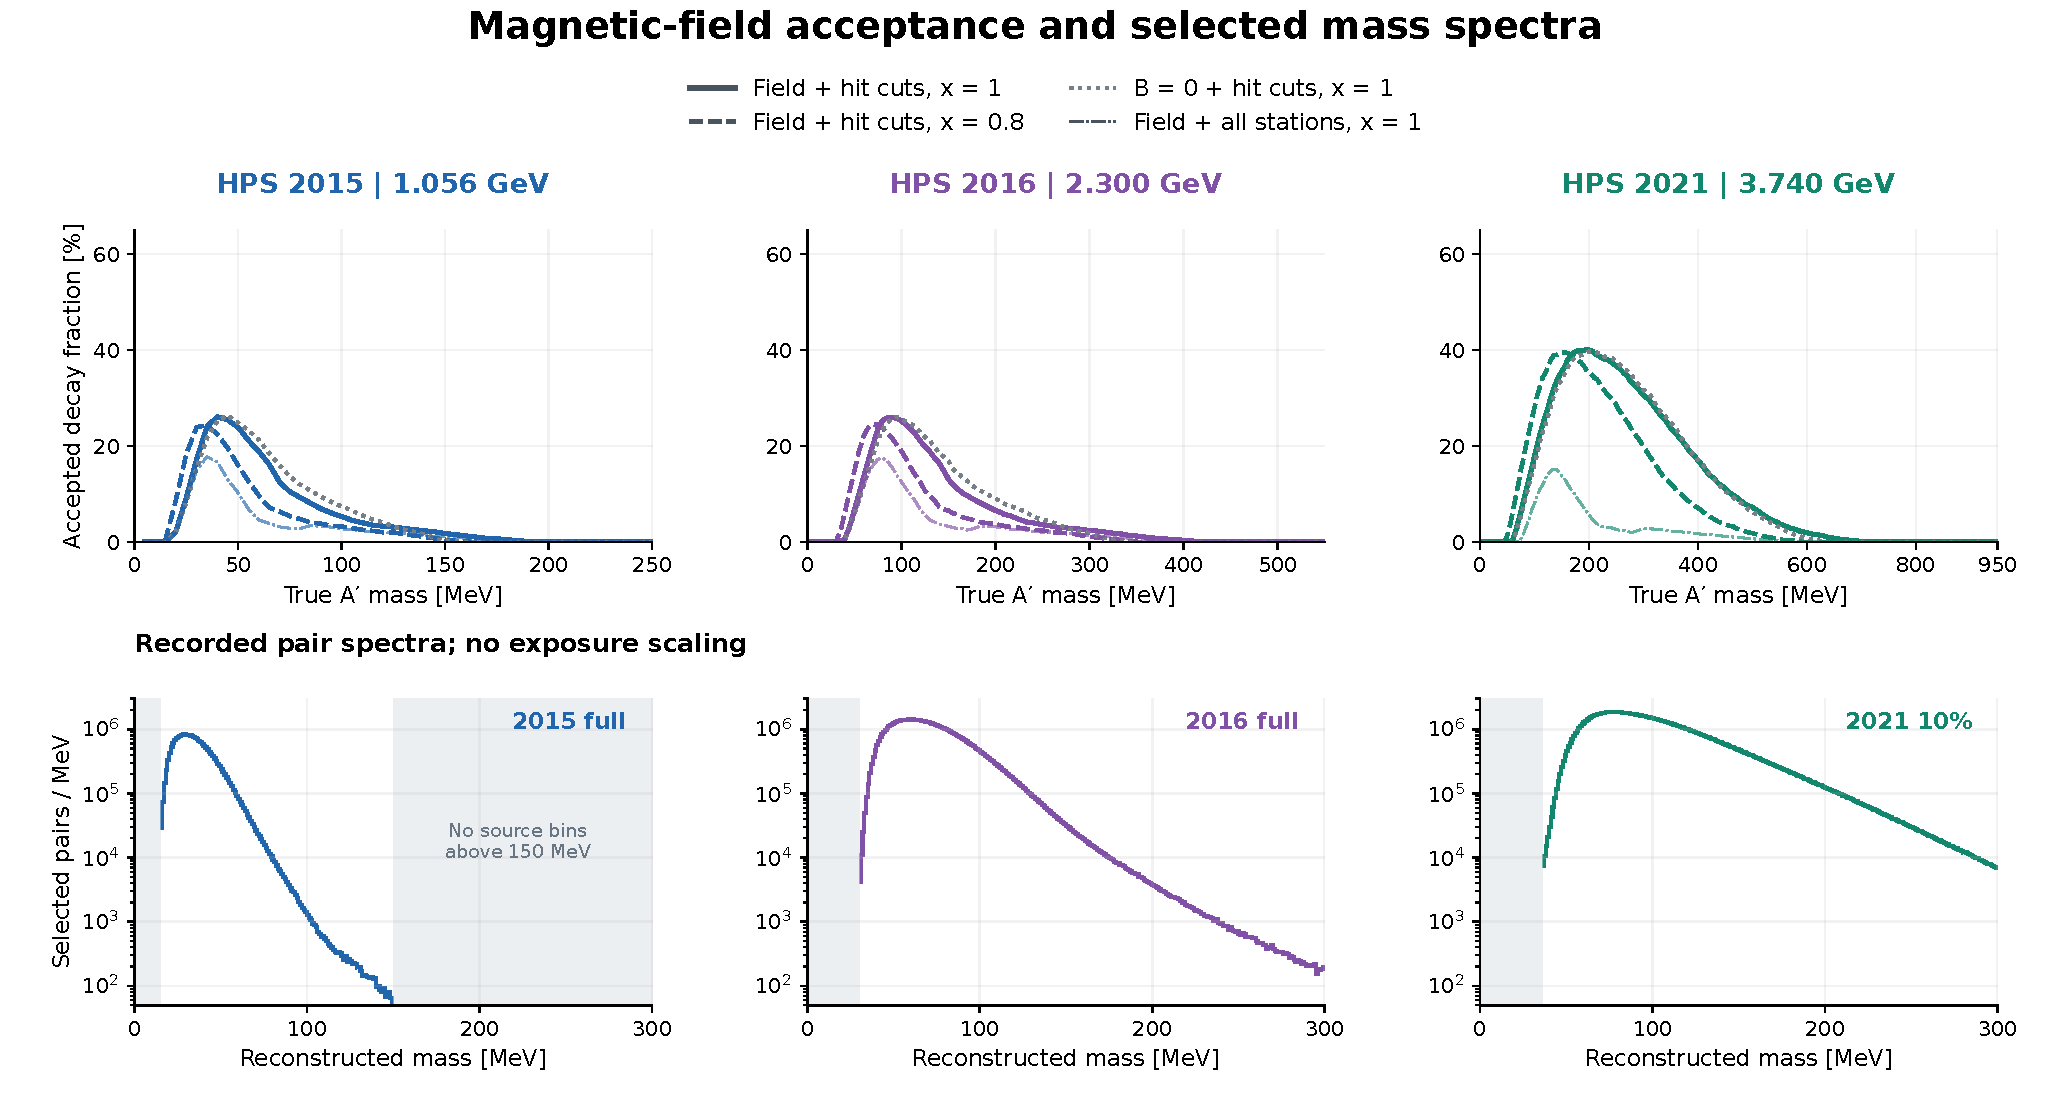
\includegraphics[width=\linewidth]{../figures/HPS_v5p7p1_response_spectra.pdf}
\caption{Conditional geometry fractions and the separately measured selected
pair spectra. The spectra retain their native exposures and selections;
their shapes and integrals are not signal efficiencies or production rates.}
\label{v571:spectra}\end{figure}
